\section{Strategische Führung / \emph{Balanced Scorecard}}
\label{sec:balanced}
Die erste Säule der Strategie für das laufende Geschäftsjahr ist die Markteinführung des Produkts am amerikanischen Markt sowie die Stärkung der Position am heimischen Markt. Durch die Stärkung am heimischen Markt soll der bestehende Marktanteil verteidigt und sogar vergrößert werden, wobei die Beziehungen zu den Bestandskunden dabei helfen werden neue Kunden am heimischen Markt zu akquirieren.
\newline
\newline
Die zweite Säule der Strategie ist die Reduzierung der Prozesskosten und der Prozesslaufzeiten, die durch Optimierungen und Automatisierungen erreicht werden soll. Damit soll der Ressourcenaufwand minimieren werden, um Kapazitäten produktiver einsetzten zu können.
\newline
\newline
Die dritte Säule der Strategie ist die stetige Verbesserung der Software und das Finden neuer Produkte und neuer Funktionalitäten der Bestandssoftware. Dadurch soll Inovationsvorsprung gegenüber den Konkurrenten ausgebaut werden. Dies soll durch mehr Fortbildungen, Motivation der Mitarbeiter und die Verwendung neuer Technologien und der Optimierung der Entwicklungsprozesse erreicht werden.

\section{Balanced Scorecard}
\bgroup
\def\arraystretch{1.5}%  1 is the default, change whatever you need
\begin{tabularx}{\textwidth}{ X | X | X | X }
	\hline
	\textbf{Ziele} & \textbf{Kennzahl} & \textbf{Maßnahmen} & \textbf{Vorgabe} \\ \hline
	
	\multicolumn{4}{p{300pt}}{\textbf{Finanzperspektive}} \\ \hline
	
	Profitabilität erhöhen  &
	Preis pro Gigabyte & 
	Dokumentenmanagement System von \emph{clever\textbf{cure}} in \emph{Cloud} auslagern  
	& Reduktion der Kosten um $25\%$ \\ \hline
	
	Marktanteil erhöhen &
	Umsatz &
	Beziehungen zu Bestandskunden verwenden um neue Kunden am Heimatmarkt zu akquirieren, sowie über Analysen fremder Märkte neue Absatzmärkte erschließen.  &
	Umsatzsteigerung um $15\%$ \\ \hline
	
	\multicolumn{4}{p{300pt}}{\textbf{Kundenperspektive}} \\ \hline
	Kundenzufriedenheit steigern & 
	\emph{Support}-Kosten &
	Schulungskosten senken in dem der Anteil an verfügbaren Schulungsvideos erhöht wird &
	Kostenreduktion um $10\%$ \\ \hline
	
	Geringerer Installationsaufwand &
	Zeitaufwand &
	Bessere Unterstützung der \emph{ERP}-System Integration unserer Softwarekomponenten &
	Zeitaufwand von 3 Tagen auf 2 Tage reduzieren \\ \hline  
	
	Benutzerfreundlichkeit erhöhen &
	Anzahl unterstützter Module &
	Unterstützung von Push-Nachrichten auf die Handys der Benutzer &
	1 Modul pro Monat \\ \hline  
	
	\multicolumn{4}{p{300pt}}{\textbf{Prozessperspektive}} \\ \hline
	Softwarequalität steigern & 
	Anzahl gefundener Bugs &
	Durch bessere interne Kommunikation, Schulungen und Fortbildungen die Fertigkeiten der Programmierer verbessern  &
	Anzahl der Programmierfehler um $20\%$ minimieren \\ \hline
	
	Einführung von \emph{Continuous deployment} &
	Zeitdauer bis \emph{release} &
	Erweitern des bestehenden \emph{Continuous integration} &
	\emph{Release}-Zeit um $30\%$ reduzieren \\ \hline 
	
	Ressourcenknappheit vermeiden &
	Anzahl der Schaltungen von Stellenausschreibungen &
	Die Stellenausschreibungen in mehreren verschiedenen Medien veröffentlichen &
	Mindestens 10 \\ \hline
	
	\multicolumn{4}{p{300pt}}{\textbf{Potentialperspektive}} \\ \hline
	Mitarbeitermotivation steigern &
	Anzahl von Zertifizierungen pro Jahr &
	Mitarbeiter motivieren sich für verwendete Software zertifizieren zu lassen &
	1 pro Jahr \\ \hline
	
	Innovationsförderung &
	Anzahl von Verbesserungsvorschlägen &
	Durch finanzielle Anreize in Form von Prämien für Verbesserungsvorschläge, die Mitarbeiter motivieren neue Anwendungsgebiete für bestehen Softwarekomponenten zu finden &
	Mindestens 3 pro Jahr \\ \hline
	
	Interne Fortbildungen steigern &
	Anzahl von Events für Schulungen &
	Durch verbesserte Organisation und Planung die Anzahl und Qualität von Schulungen steigern &
	5 pro Jahr \\ \hline
	
\end{tabularx}
\egroup
\ \newpage
\subsection{BSC-Waage}
In diesem Abschnitt ist die aufgestellte BSC-Waage angeführt.
\begin{figure}[h]
	\centering
	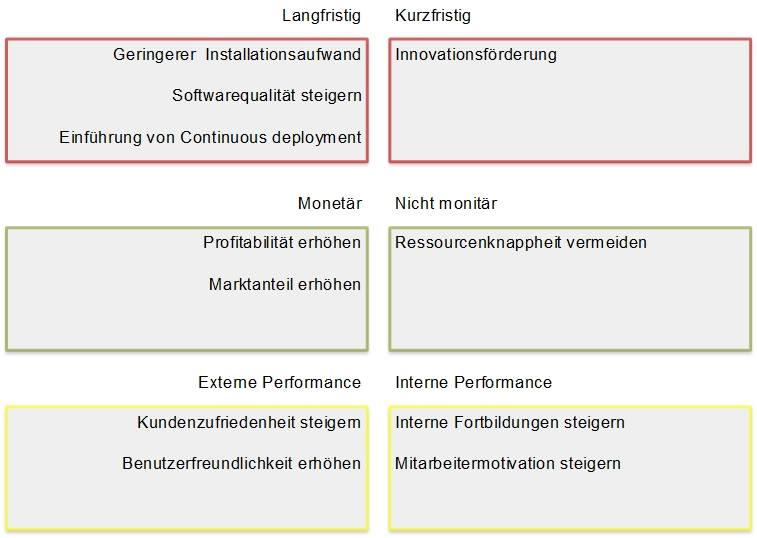
\includegraphics[scale=0.82]{\imageDir/waage.jpg}
	\caption{BSC-Waage}
	\label{fig:balanced-bsc}
\end{figure}
\ \newpage
\subsection{Treiberbaum}
In diesem Abschnitt ist der aufgestellte Treiberbaum angeführt.
\begin{figure}[h]
	\centering
	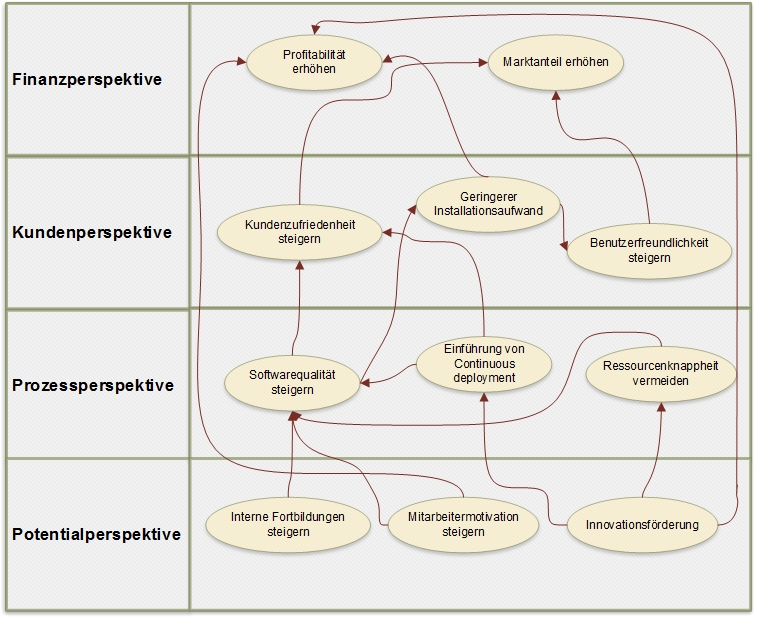
\includegraphics[scale=0.82]{\imageDir/tree.jpg}
	\caption{Treiberbaum}
	\label{fig:balanced-tree}
\end{figure}
\subsubsection{Erläuterung des Treiberbaums}
Durch die Fortbildungen der Mitarbeiter und die Mitarbeitermotivation wird die Softwarequalität und die Profitabilität gesteigert. Durch die gesteigerte Kundenzufriedenheit wird der Marktanteil verteidigt und ebenso erhöht, da die zufriedenen Kunden dem Unternehmen helfen neue Kunden zu akquirieren.
\newline
\newline
Durch die Steigerung der Innovation wird die Einführung von \emph{Continuous integration} ermöglicht, sowie die Gefahr von Ressourcenknappheit minimiert, da ein innovatives Unternehmen bessere Chancen hat neue Mitarbeiter zu gewinnen, sowie bestehende Mitarbeiter im Unternehmen zu halten. Gleichermaßen wird die Softwarequalität durch Innovationen und durch die geringe Gefahr einer Ressourcenknappheit gefördert.
\newline
\newline
Das \emph{Continuous deployment} fördert die Kundenzufriedenheit durch schnellere Releases und fördert auch die Softwarequalität durch bessere Integration der Softwareentwicklung in den \emph{Build} und \emph{Release}-Prozess. Die Steigerung der Benutzerfreundlichkeit wird durch eine Minimierung des Installationsaufwandes erreicht was natürlich die Kundenzufridenheit positiv beeinflusst.
